\documentclass{beamer}

\usepackage[T1]{fontenc}
\usepackage[utf8]{inputenc}
\usepackage[american]{babel}
\usepackage{amsmath,amssymb,amsthm}
\usepackage{tikz}
\usepackage[backend=biber,citestyle=authoryear-comp,bibstyle=beamer,doi=false,isbn=false,url=false,maxnames=10]{biblatex}
\bibliography{defeo}
\usepackage[nosfdefault]{comicneue}

\mode<presentation>{%
  \usetheme{Boadilla}
}
\beamertemplatenavigationsymbolsempty
\usecolortheme[RGB={110,117,124}]{structure}
\setbeamercolor*{title}{fg=white!50!black}
\setbeamercolor*{titlegraphic}{fg=white!20!black}

\usepackage{sourcesanspro}
\usepackage[amssymb,amsfonts]{concmath}
\usefonttheme[onlymath]{serif}

\renewcommand{\emph}[1]{{\usebeamercolor[fg]{structure}#1}}

%\let\footcite\footnote

\newcommand{\C}{\mathbb{C}}
\newcommand{\R}{\mathbb{R}}
\newcommand{\Z}{\mathbb{Z}}
\newcommand{\N}{\mathbb{N}}
\newcommand{\Q}{\mathbb{Q}}
\newcommand{\F}{\mathbb{F}}
\renewcommand{\O}{\mathcal{O}}
\newcommand{\tildO}{\mathcal{\tilde{O}}}
\newcommand{\End}{\operatorname{End}}
\newcommand{\chr}{\operatorname{char}}
\newcommand{\Cl}{\operatorname{Cl}}
\renewcommand{\a}{{\mathfrak{a}}}
\renewcommand{\b}{{\mathfrak{b}}}
\newcommand{\cyc}[1]{{\langle #1 \rangle}}
\newcommand{\ord}{\operatorname{ord}}

\usetikzlibrary{matrix,decorations,decorations.text,calc,arrows,snakes,shapes,positioning}

\pgfkeys{/triangle/.code=\tikzset{x={(-0.5cm,-0.866cm)},y={(1cm,0cm)}}}
\pgfkeys{/lattice/.code n args={4}{\tikzset{cm={#1,#2,#3,#4,(0,0)}}}}

\newcommand{\axes}[4]{
  \clip (#1,#3) rectangle (#2,#4);
  \draw [thin, gray, -latex] (#1,0) -- (#2,0);% Draw x axis
  \draw [thin, gray, -latex] (0,#3) -- (0,#4);% Draw y axis
}

\newcommand{\lattice}[2]{
  \draw[style=help lines,dashed] (#1-1,#1-1) grid[step=1] (#2+1,#2+1);
  \foreach \x in {#1,...,#2}{
    \foreach \y in {#1,...,#2}{
      \node[draw,circle,inner sep=2pt,fill] at (\x,\y) {};
      % Places a dot at those points
    }
  }
}

\newcommand{\bl}[1]{\textcolor{blue}{#1}}
\newcommand{\rd}[1]{\textcolor{red}{#1}}
\newcommand{\gr}[1]{\textcolor{green}{#1}}

% This command defines a triangle of dots of given height
\newcommand{\dottriangle}[2][\i-\j]{%
  \foreach \i in {0,...,#2} {%
    \foreach \j in {0,...,\i} {%
      \draw(\i,\j) node{#1};%
    }%
  }}


\title[Key exchange from isogeny graphs]{Key exchange from isogeny graphs: ordinary or supersingular?}
\author[Luca De Feo]{Luca De Feo\\
  \footnotesize hand-drawings by Rachel Deyts}
\date[July 11, 2018, Microsoft]{July 11, 2018, Microsoft Research}
\institute[UVSQ \& INRIA]{Université de Versailles \& Inria, Université Paris-Saclay}

\begin{document}

\frame[plain]{
  \begin{tikzpicture}[overlay]
    \node[opacity=0.2] at (10,5) {
      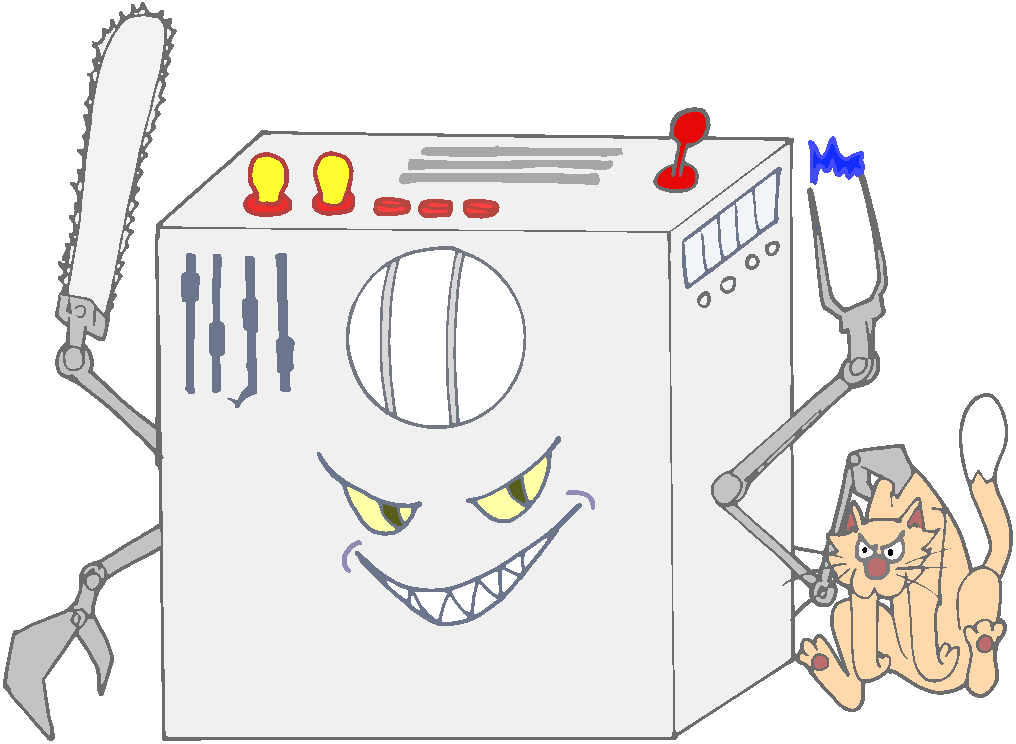
\includegraphics[height=4\textheight]{qc-color}
    };
  \end{tikzpicture}
  \vspace{-2.5cm}
  \usebeamercolor[fg]{titlegraphic}
  {\bf \titlepage}
}

%% 

\begin{frame}{Elliptic curves}

  Let \emph{$E \;:\; y^2 = x^3 + ax + b$} be an elliptic curve\dots

  \begin{center}
    \begin{tikzpicture}[domain=-2.4566:4,samples=100]
      \newcount\rotate
      \animate<2-6>
      \animatevalue<2-6>{\rotate}{0}{90}
      \begin{scope}[rotate=-\the\rotate]
        \draw plot (\x,{0.5*sqrt(\x*\x*\x-4*\x+5)});
        \draw plot (\x,{-0.5*sqrt(\x*\x*\x-4*\x+5)});
      \end{scope}
      
      \begin{uncoverenv}<1>
        \begin{scope}[yscale=1/2]
          \draw[thin,gray,-latex] (0,-7) -- (0,7);
          \draw[thin,gray,-latex] (-3,0) -- (4,0);
          
          \draw (-3,1) -- (4,8/3+3);
          \begin{scope}[every node/.style={draw,circle,inner sep=1pt,fill},cm={1,2/3,0,0,(0,3)}]
            \node at (-2.287980,0) {};
            \node at (-0.535051,0) {};
            \node at (3.267475,0) {};
          \end{scope}
          \begin{scope}[every node/.style={yshift=0.3cm},cm={1,2/3,0,0,(0,3)}]
            \node at (-2.287980,0) {$P$};
            \node at (-0.535051,0) {$Q$};
            \node at (3.267475,0) {$R$};
          \end{scope}
          \draw[dashed] (3.267475,3.267475*2/3+3) -- (3.267475,-3.267475*2/3-3) 
          node[draw,circle,inner sep=1pt,fill] {}
          node[xshift=-0.1cm,anchor=east] {$P+Q$};
        \end{scope}
      \end{uncoverenv}
    \end{tikzpicture}
  \end{center}
\end{frame}

%%

\begin{frame}{Elliptic curves}
  \transdissolve
  \centering

  \bigskip
  
  
\includegraphics[height=0.7\textheight]{ec-happy}

  \Large\bf I power 70\% of WWW traffic!
\end{frame}

%%

\begin{frame}{The QUANTHOM Menace}
  \centering
  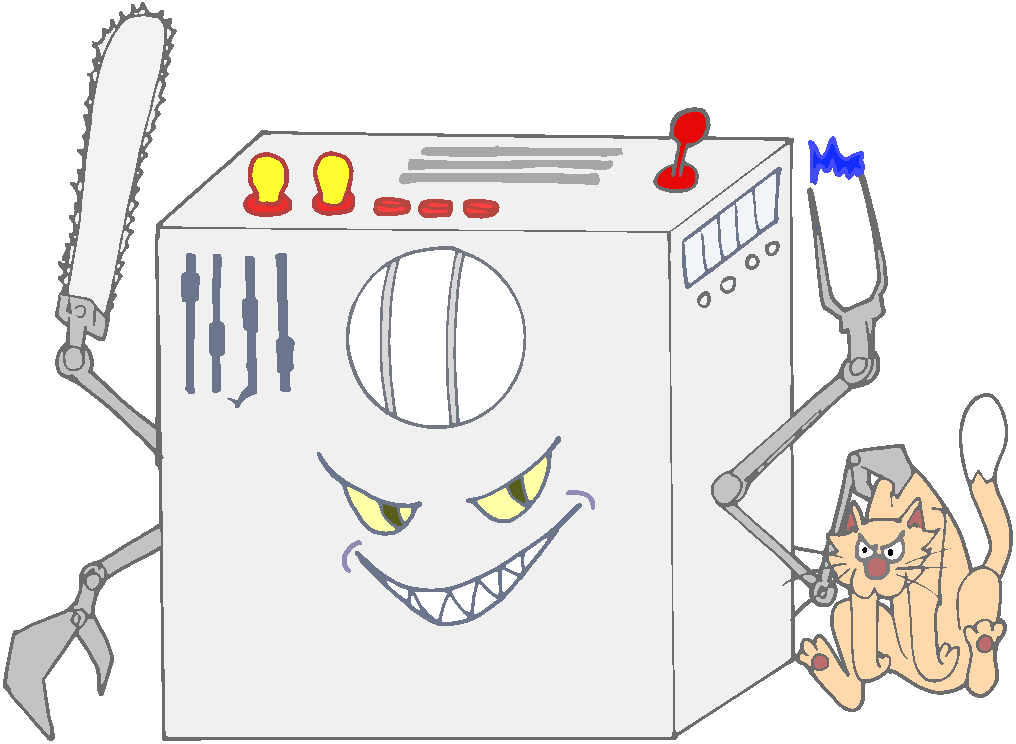
\includegraphics[height=0.7\textheight]{qc-color}
\end{frame}

%%

\begin{frame}{Post-quantum cryptographer?}
  \centering
  \includegraphics[height=0.7\textheight]{ec-broke}
\end{frame}

%%

\begin{frame}{Elliptic curves of the world, UNITE!}
  \centering
  \begin{tikzpicture}
    \foreach \x/\y in {0/-0.5,4/2,8/-1}{
      \node at (\x,\y) {\includegraphics[height=3cm]{ec-banderole}};
    }
    \foreach \x/\y in {1/3,4.5/-1,7/3}{
      \node at (\x,\y) {
\includegraphics[height=3.5cm]{ec-sign}};
    }
    \color{teal!70!blue}\itshape\bfseries\comicneue
    \node[rotate=-3] at (5.9,3.6) {\parbox{0pt}{QUOUSQUE\\QUANTUM?}};
    \node[rotate=-3] at (3.6,-0.4) {\parbox{0pt}{QUANTUM\\SUFFICIT!}};
  \end{tikzpicture}
\end{frame}

%%

\begin{frame}{And so, they found a way around the Quanthom...}
  \centering
  \begin{tikzpicture}
    \comicneue\itshape
    \node at (0,0) {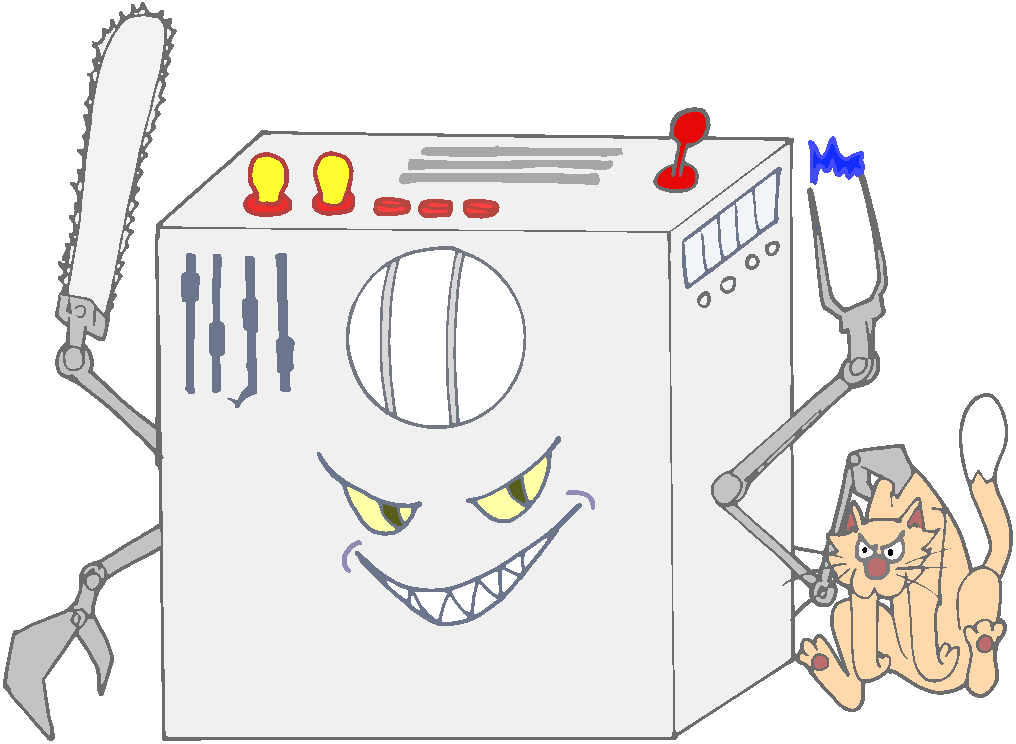
\includegraphics[height=2.5cm]{qc-color}};
    
    \node(E0) at (-5,0) {
\includegraphics[height=1cm]{ec-happy}};

    \uncover<2->{
      \node(EA) at (0,3.5) {
\includegraphics[height=1cm]{ec-happy}};
      \node(EB) at (0,-3.5) {
\includegraphics[height=1cm]{ec-happy}};
      \draw[->,decorate,decoration=snake] (E0) to (EA);
      \draw[->,decorate,decoration=snake] (E0) to (EB);
      \node[right=0.3cm of EA] {\bl{Public curve}};
      \node[right=0.3cm of EB] {\bl{Public curve}};
    }
    \uncover<3>{
      \node(ES) at (5,0) {
\includegraphics[height=1cm]{ec-happy}};
      \draw[->,decorate,decoration=snake] (EA) to (ES);
      \draw[->,decorate,decoration=snake] (EB) to (ES);
      \node[below=1em of ES] {\rd{Shared secret}};
    }
  \end{tikzpicture}
\end{frame}

%%

\begin{frame}{What's an isogeny?}
  \centering
  
\includegraphics[height=2cm]{ec-happy}
  \hfill
  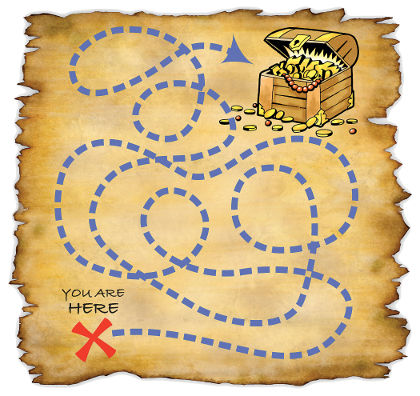
\includegraphics[height=4cm]{map}
  \hfill
  
\includegraphics[height=2cm]{ec-happy}

  \bigskip
  \Large Rebus: 1-3-7-3-8-6
\end{frame}

%%


\begin{frame}
  \frametitle{Elliptic curves over $\C$}

  \begin{columns}
    \begin{column}{0.75\textwidth}
      \begin{tikzpicture}[scale=2]
        \axes{-1}{3.5}{-0.5}{3}

        \begin{scope}[/lattice={1}{0.2}{0.4}{0.7}]
          \begin{uncoverenv}<1>
            \draw[fill,black!10] (0,0) -- (1,0) -- (1,1) -- (0,1) -- (0,0);
            \node at (0.5,0.5) {$\C/\Lambda$};
            \node at (0.9,-0.1) {$\omega_1$};
            \node at (-0.1,0.9) {$\omega_2$};
          \end{uncoverenv}

          \lattice{-3}{4}

          \begin{uncoverenv}<2-5>
            \node[red] at (0.7,0.65) {$a$}; 
            \node[draw,circle,inner sep=1pt,fill,red] at (0.8,0.5) {};
            \node[red] at (0.2,0.9) {$b$}; 
            \node[draw,circle,inner sep=1pt,fill,red] at (0.3,0.7) {};
            
            \begin{uncoverenv}<3-4>
              \node[red] at (1.2,1.3) {$a+b$}; 
              \node[draw,circle,inner sep=1pt,fill,red] at (1.1,1.2) {};
              \begin{uncoverenv}<3>
                \draw[red,thin] (0,0) -- (0.8,0.5) -- (1.1,1.2);
                \draw[red,thin] (0,0) -- (0.3,0.7) -- (1.1,1.2);          
              \end{uncoverenv}
            \end{uncoverenv}

            \transdissolve<5>
            \begin{uncoverenv}<5>
              \node[red] at (0.2,0.3) {$a+b$}; 
              \node[draw,circle,inner sep=1pt,fill,red] at (0.1,0.2) {};
            \end{uncoverenv}
          \end{uncoverenv}
        \end{scope}  
      \end{tikzpicture}
    \end{column}
    \begin{column}{0.2\textwidth}
      \begin{onlyenv}<1>
        Let $\omega_1,\omega_2\in\C$ be linearly independent complex
        numbers. Set
        \[\emph{\Lambda = \omega_1\Z \oplus \omega_2\Z}\]

        $\C/\Lambda$ is an elliptic curve.
      \end{onlyenv}

      \begin{onlyenv}<2->
        Addition law induced by addition on $\mathbb{C}$.
      \end{onlyenv}
    \end{column}
  \end{columns}
\end{frame}

%% 

\begin{frame}
  \frametitle{Isomorphism classes}

  \begin{columns}
    \begin{column}{0.7\textwidth}
      \begin{tikzpicture}[scale=2]
        \axes{-1}{3.3}{-0.5}{3}

        \newcount\scale
        \animate<1-21>
        \animatevalue<1-21>{\scale}{0}{20}
        \begin{uncoverenv}<1-22>
          \begin{scope}[/lattice={1}{0.2}{0.4}{0.7},scale=1+\the\scale/20,rotate=\the\scale]
            \lattice{-3}{4}
            \node[red,yshift=0.2cm] at (0.8,0.5) {$a$}; 
            \node[draw,circle,inner sep=1pt,fill,red] at (0.8,0.5) {};
          \end{scope}
        \end{uncoverenv}
      \end{tikzpicture}      
    \end{column}
    \begin{column}{0.25\textwidth}
      Two lattices are \emph{homotetic} if there exist $\alpha\in\C$
      such that
      \[\emph{\alpha\Lambda_1 = \Lambda_2}\]

      The \alert{$j$-invariant} $j(\Lambda)$ classifies elliptic curves
      up to \emph{homothety} (\emph{isomorphism}).
    \end{column}
  \end{columns}
\end{frame}  

%%

\begin{frame}
  \frametitle{Multiplication}

  \begin{tikzpicture}[scale=2.2]
    \axes{-1}{4.5}{-0.5}{3}

    \begin{scope}[/lattice={1}{0.2}{0.4}{0.7}]
      \lattice{-3}{5}
    
      \node[red,yshift=0.2cm] at (0.8,0.6) {$a$}; 
      \draw[red] (0.8,0.6) node[fill,circle,inner sep=1pt] {};

      \begin{uncoverenv}<2>
        \node[red,yshift=0.2cm] at (2.4,1.8) {$[3]a$}; 
        \draw[red] (0,0) -- (1.6,1.2) node[fill,circle,inner sep=1pt] {} 
        -- (2.4,1.8) node[fill,circle,inner sep=1pt] {};
      \end{uncoverenv}

      \transdissolve<3>
      \begin{uncoverenv}<3>
        \node[red,yshift=0.3cm] at (0.4,0.8) {$[3]a$}; 
        \draw[red] (0.4,0.8) node[fill,circle,inner sep=1pt] {};
      \end{uncoverenv}
    \end{scope}
  \end{tikzpicture}
\end{frame}

%%

\begin{frame}
  \frametitle{Torsion subgroups}

  \begin{columns}
    \begin{column}{0.7\textwidth}
      \begin{tikzpicture}[scale=1.8]
        \axes{-0.3}{4.5}{-0.5}{4};

        \begin{scope}[/lattice={3}{0.6}{1.2}{2.1}]
          \lattice{-1}{2}

          \foreach \i in {0,...,2} {
            \foreach \j in {0,...,2} {
              \draw[red] (\i/3,\j/3) node[fill,circle,inner sep=1pt] {};
            }
          }
          \draw[red] (0,0) -- (1/3,0) node[yshift=0.2cm] {$a$};
          \draw[red] (0,0) -- (0,1/3) node[yshift=0.2cm] {$b$};
        \end{scope}
      \end{tikzpicture}  
    \end{column}
    \begin{column}{0.25\textwidth}
      The $\ell$-torsion subgroup is made up by the points
      \[\emph{\left(\frac{i\omega_1}{\ell},\frac{j\omega_2}{\ell}\right)}\]

      It is a group of rank two
      \begin{alertenv}
        \begin{align*}
          E[\ell] &= \langle a,b \rangle\\
          &\simeq (\Z/\ell\Z)^2
        \end{align*}
      \end{alertenv}
    \end{column}
  \end{columns}
\end{frame}

%%

\begin{frame}
  \frametitle{Isogenies}

  \begin{columns}
    \begin{column}{0.7\textwidth}
      \begin{tikzpicture}[scale=1.8]
        \axes{-0.3}{4.5}{-0.5}{4};
        
        \begin{scope}[/lattice={3}{0.6}{1.2}{2.1}]
          \uncover<1->{\lattice{-1}{2}}
          
          \begin{uncoverenv}<1-3>
            \draw[red] (0,0) -- (1/3,0) node[yshift=0.3cm] {$a$};
          \end{uncoverenv}
          \begin{uncoverenv}<4->
            \draw[red] (0,0) -- (0,1/3) node[yshift=0.3cm] {$b$};
          \end{uncoverenv}

          \begin{uncoverenv}<1-2>
            \draw[blue] (0.8,0.5) node[yshift=0.3cm] {$p$};
            \draw[blue] (0.8,0.5) node[fill,circle,inner sep=1pt] {};
          \end{uncoverenv}
        \end{scope}
        
        \begin{scope}[/lattice={1}{0.2}{1.2}{2.1}]
          \transdissolve<2>
          \begin{scope}[opacity=0.3]
            \uncover<2-4>{\lattice{-3}{5}}
          \end{scope}
          
          \transdissolve<3>
          \begin{uncoverenv}<3-5>
            \draw[blue] (0.4,0.5) node[yshift=0.3cm] {$p$};
            \draw[blue] (0.4,0.5) node[fill,circle,inner sep=1pt] {};
          \end{uncoverenv}
        \end{scope}

        \begin{scope}[/lattice={1}{0.2}{0.4}{0.7}]
          \transdissolve<5>
          \begin{scope}[opacity=0.3]
            \uncover<5->{\lattice{-3}{5}}
          \end{scope}
          
          \transdissolve<6>
          \begin{uncoverenv}<6->
            \draw[blue] (0.4,0.5) node[yshift=0.3cm] {$p$};
            \draw[blue] (0.4,0.5) node[fill,circle,inner sep=1pt] {};
          \end{uncoverenv}
        \end{scope}
        
        \begin{scope}[/lattice={3}{0.6}{1.2}{2.1}]
          \foreach \i in {0,...,2} {
            \foreach \j in {0,...,2} {
              \draw[red] (\i/3,\j/3) node[fill,circle,inner sep=1pt] {};
            }
          }
        \end{scope}
      \end{tikzpicture}  
    \end{column}
    \begin{column}{0.25\textwidth}
      \begin{onlyenv}<1-3>
        Let $\rd{a}\in\C/\Lambda_1$ be an $\ell$-torsion point, and let
        \[\emph{\Lambda_2 = a\Z\oplus\Lambda_1}\]
        Then \emph{$\Lambda_1\subset\Lambda_2$} and we define a degree
        $\ell$ cover
        \[\emph{\phi:\C/\Lambda_1\to\C/\Lambda_2}\]

        \emph{$\phi$} is a morphism of complex Lie groups and is called an
        \alert{isogeny}.
      \end{onlyenv}
      \begin{onlyenv}<4-> 
        Taking a point $\rd{b}$ not in the kernel of \emph{$\phi$}, we
        obtain a new degree $\ell$ cover
        \[\emph{\hat{\phi}:\C/\Lambda_2\to\C/\Lambda_3}\]

        The composition \emph{$\hat{\phi}\circ\phi$} has degree
        $\ell^2$ and is \alert{homothetic to the multiplication} by
        $\ell$ map.

        \emph{$\hat{\phi}$} is called the \alert{dual isogeny} of
        \emph{$\phi$}.
      \end{onlyenv}
    \end{column}
  \end{columns}
\end{frame}

%%

\begin{frame}
  \frametitle{Isogenies}

  Isogenies are just \alert{the right notion\texttrademark{} of
    morphism} for elliptic curves

  \begin{itemize}
  \item Surjective group morphisms.
  \item Algebraic maps (i.e., defined by polynomials).
  \end{itemize}

  (Separable) isogenies $\Leftrightarrow$ finite subgroups:
  \alert{\[0 \to H \to E \overset{\phi}{\to} E' \to 0\]}
  The kernel \emph{$H$} determines the image curve \emph{$E'$} up to
  isomorphism \[\emph{E/H\overset{\text{\tiny def}}{=}E'}.\]

  \begin{block}{Isogeny degree}
    Neither of these definitions is quite correct, but they
    \textit{nearly} are:
    \begin{itemize}
    \item The degree of \emph{$\phi$} is the cardinality of \emph{$\ker\phi$}.
    \item (\emph{Bisson}) the degree of \emph{$\phi$} is the time
      needed to compute it.
    \end{itemize}
  \end{block}
\end{frame}

%%

\begin{frame}{Isogenies: an example over $\F_{11}$}
  \begin{tikzpicture}[scale=0.4]
    \begin{scope}
      \node[anchor=center] at (0,7) {$E \;:\; y^2 = x^3 + x$};

      \uncover<-1>{
        \draw[thin,gray] (0,-6) -- (0,6);
        \draw[thin,gray] (-6,0) -- (6,0);
      }

      \foreach \x/\y in {0/0,5/3,-4/3,-3/5,-2/1,-1/3} {
        \draw[blue,fill] (\x,\y) circle (0.2) node(E_\x_\y){}
        (\x,-\y) circle (0.2) node(E_\x_-\y){};
      }

      \uncover<4->{\draw[red,fill] (0,0) circle (0.3);}
    \end{scope}

    \draw[black!10!white,thick] (8,-7) -- +(0,14);
    
    \begin{scope}[shift={(16,0)}]
      \node at (0,7) {$E' \;:\; y^2 = x^3 - 4x$};

      \uncover<-1>{
        \draw[thin,gray] (0,-6) -- (0,6);
        \draw[thin,gray] (-6,0) -- (6,0);
      }

      \foreach \x/\y in {0/0,2/0,3/2,4/2,6/4,-2/0,-1/5} {
        \draw[color=blue,fill] (\x,\y) circle (0.2) node(F_\x_\y){}
        (\x,-\y) circle (0.2) node(F_\x_-\y){};
      }
    \end{scope}

    \begin{scope}[color=red,-latex,dashed]
      \begin{uncoverenv}<2->
        \path
        (E_5_3) edge (F_3_2)
        (E_-4_3) edge (F_4_-2)
        (E_-3_5) edge (F_4_2)
        (E_-2_1) edge (F_3_-2)
        (E_-1_3) edge (F_-2_0);
      \end{uncoverenv}
      \begin{uncoverenv}<2,5->
        \path
        (E_5_-3) edge (F_3_-2)
        (E_-4_-3) edge (F_4_2)
        (E_-3_-5) edge (F_4_-2)
        (E_-2_-1) edge (F_3_2)
        (E_-1_-3) edge (F_-2_0);
      \end{uncoverenv}
    \end{scope}
  \end{tikzpicture}
  
  \begin{columns}
    \begin{column}{0.5\textwidth}
      \[\phi(x,y) = \left(\frac{x^2 + 1}{x},\quad y\frac{x^2-1}{x^2}\right)\]
    \end{column}
    \begin{column}{0.5\textwidth}
      \begin{itemize}
      \item<4-> Kernel generator in \alert{red}.
      \item<5-> This is a degree $2$ map.
      \item<6-> Analogous to $x\mapsto x^2$ in $\F_q^*$.
      \end{itemize}
    \end{column}
  \end{columns}
\end{frame}

%%

\begin{frame}{Computing isogenies 101: Vélu's formulas}
  \begin{description}
  \item[Input:] A subgroup \emph{$H\subset E(k)$}.
  \item[Output:] The rational fractions defining \emph{$\phi:E\to E/H$}.
  \end{description}

  \begin{align*}
    \phi(P) = \Bigl(
    &x(P) + \sum_{Q\in H\setminus\{\O\}}x(P+Q)-x(Q),\\
    &y(P) + \sum_{Q\in H\setminus\{\O\}}y(P+Q)-y(Q)
      \Bigr);
  \end{align*}

  And \emph{$E/H$} has equation \emph{$y^2=x^3+a'x+b'$}, where
  
  \begin{align*}
    a' &= a - 5\sum_{Q\in H\setminus\{\O\}}(3x(Q)^2+a),\\
    b' &= b - 7\sum_{Q\in H\setminus\{\O\}}(5x(Q)^3+3ax(Q)+b).
  \end{align*}

  \begin{description}
  \item[Complexity:] $\tildO(\# H)$ operations in $k$.
  \end{description}
\end{frame}

%%

\begin{frame}{Computing isogenies 102: Elkies' algorithm (and variants)}
  \begin{description}
  \item[Input:] An elliptic curve \emph{$E$} defined over $k$, a
    prime \emph{$\ell$}.
  \item[Output:]
    \begin{itemize}
    \item One (all) curve such that there exists \emph{$\phi:E\to E'$}
      of degree \emph{$\ell$},
    \item The corresponding rational fractions.
    \end{itemize}
  \item[Idea:]
    \begin{itemize}
    \item The \textbf{modular polynomial} \emph{$\Phi_\ell\in\Z[X,Y]$}
      encodes all the information on isogenies of degree $\ell$;
    \item \textbf{Evaluate} \emph{$\Phi_\ell(j(E),Y)$};
    \item \textbf{Factor} it over \emph{$k[Y]$} to find all isogenous
      elliptic curves of degree $\ell$;
    \item \textbf{Recover} the rational fractions (\textit{easy}).
    \end{itemize}
  \item[Complexity:] \alert{$\tildO(\ell^2 + \ell\log q)$ operations
      in $k=\F_q$.} \emph{(yes, that's a lot!)}
  \end{description}
\end{frame}

%%

\begin{frame}
  \frametitle{Isogeny graphs}
  
  \vspace{-2mm}

  \begin{columns}
    \begin{column}{0.65\textwidth}
      We look at the graph of elliptic curves with isogenies \emph{up
        to isomorphism}.  We say two \alert{isogenies} $\phi,\phi'$
      are \alert{isomorphic} if:
    \end{column}
    \begin{column}{0.3\textwidth}
      \begin{center}
        \begin{tikzpicture}[node distance=4em]
          \node(E){$E$}; 
          \node(E1)[right of=E]{$E'$};
          \node(E2)[below of=E1]{$E'$};
          \scriptsize
          \path[->] (E) edge node[auto]{$\phi$} (E1);
          \path[->] (E) edge node[auto,swap]{$\phi'$} (E2);
          \path[<->] (E1) edge node[rotate=270] {\large$\widetilde{}$} (E2);
        \end{tikzpicture}
      \end{center}
    \end{column}
  \end{columns}

  \emph{Example:} Finite field, ordinary case, graph of isogenies of degree $3$.

  \begin{center}
    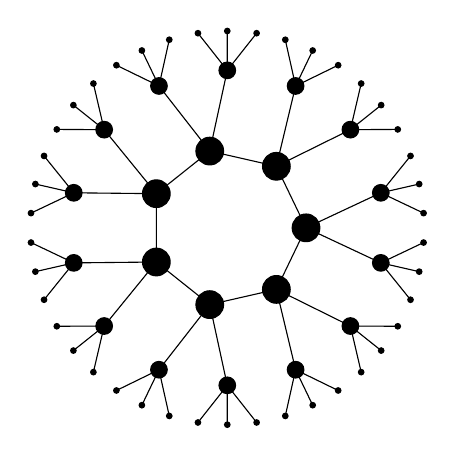
\begin{tikzpicture}[]
      \begin{scope}
        \def\crater{7}
        \foreach \i in {1,...,\crater} {
          \draw[fill] (360/\crater*\i:1cm) circle (5pt);
          \draw (360/\crater*\i : 1cm) -- (360/\crater*\i+360/\crater : 1cm);
          \foreach \j in {-1,1} {
            \draw[fill] (360/\crater*\i : 1cm) -- (360/\crater*\i + \j*360/\crater/4 : 2cm) circle (3pt);
            \foreach \k in {-1,0,1} {
              \draw[fill] (360/\crater*\i + \j*360/\crater/4 : 2cm) --
              (360/\crater*\i + + \j*360/\crater/4 + \k*360/\crater/6 : 2.5cm) circle (1pt);
            }
          }
        }
      \end{scope}
    \end{tikzpicture}
  \end{center}
\end{frame}

%%

\begin{frame}
  \frametitle{Structure of the graph\footcite{deuring41,kohel,fouquet+morain02,DelfsG16}}
  
  \begin{theorem}[Serre-Tate]
    Two curves are isogenous over a finite field $k$ if and only if
    they have the \alert{same number of points} on $k$.
  \end{theorem}
  \vspace{-0.6em}
  \begin{block}{The graph of isogenies of \alert{prime} degree \alert{$\ell\ne p$}}
    \small
    \vspace{-1em}
    \begin{tabular}{p{0.17\textwidth} p{0.8\textwidth}}
      \raggedright
      \emph{Ordinary case (isogeny volcanoes)}
      & \vspace{-1em}
        \begin{itemize}
          \setlength\itemsep{-0.6ex}
        \item Nodes can have degree \emph{$0,1,2$} or \emph{$\ell+1$}.
          \begin{itemize}
          \item  For $\sim 50\%$ of the primes $\ell$, graphs are just isolated
            points;
          \item For other $\sim 50\%$, graphs are $2$-regular;
          \item other cases only happen for finitely many $\ell$'s.
          \end{itemize}
        \end{itemize}
      \\[-1em]
      \raggedright
      \emph{Supersingular case ($\F_p$)}
      & \vspace{-1em}
        \begin{itemize}
          \setlength\itemsep{-0.6ex}
        \item If $\ell=2$ nodes have degree $1$, $2$ or $3$;
        \item For any other $\ell$, graphs are $2$-regular.
        \end{itemize}
      \\[-1em]
      \raggedright
      \emph{Supersingular case ($\F_{p^2}$)}
      & \vspace{-1em}
        \begin{itemize}
          \setlength\itemsep{-0.6ex}
        \item The graph is \emph{$\ell+1$-regular}.
        \item There is a \alert{unique (finite) connected component} made
          of all supersingular curves with the same number of points.
        \end{itemize}
    \end{tabular}
    \vspace{-1.5em}
  \end{block}
\end{frame}

%%

\begin{frame}{Expander graphs from isogenies}
  \begin{block}{Expander graphs}
    An infinite family of connected $k$-regular graphs on $n$ vertices
    is an \emph{expander family} if there exists an $\epsilon>0$ such
    that all \emph{non-trivial} eigenvalues satisfy
    $|\lambda| \le (1-\epsilon)k$ for $n$ large enough.
    \begin{itemize}
    \item Expander graphs have \emph{short diameter} ($O(\log n)$);
    \item Random walks \emph{mix rapidly} (after $O(\log n)$ steps,
      the induced distribution on the vertices is close to uniform).
    \end{itemize}
  \end{block}

  \begin{description}
  \item[Supersingular] Let $\ell$ be fixed, the graphs of all supersingular curves
    with $\ell$-isogenies are expanders;\footcite{pizer1,pizer2}
  \item[Ordinary*] Let $\O\subset\Q[\sqrt{-D}]$ be an order in a
    quadratic imaginary field. The graphs of all curves over $\F_q$
    with \emph{complex multiplication by $\O$}, with isogenies of
    prime degree bounded by $(\log q)^{2+\delta}$, are
    expanders.\footcite{jao+miller+venkatesan09} \hfill{\tiny *(may contain traces of GRH)}
  \end{description}
\end{frame}

%%

\begin{frame}
  \frametitle{Expander graphs from groups}
  \begin{center}
    \begin{tikzpicture}
      \begin{scope}
        \def\crater{12}
        \def\jumpa{-8}
        \def\jumpb{9}
        \def\diam{3cm}

        \foreach \i in {1,...,\crater} {
          \uncover<2->{\draw[blue] (360/\crater*\i : \diam) to[bend right] (360/\crater*\i+360/\crater : \diam);}
          \uncover<3->{\draw[red] (360/\crater*\i : \diam) to[bend right] (360/\crater*\i+\jumpa*360/\crater : \diam);}
          \uncover<4->{\draw[green] (360/\crater*\i : \diam) to[bend right=50] (360/\crater*\i+\jumpb*360/\crater : \diam);}
        }
        \foreach \i in {1,...,\crater} {
          \pgfmathparse{int(mod(2^\i,13))}
          \let\exp\pgfmathresult
          \draw[fill] (360/\crater*\i: \diam) circle (2pt) +(360/\crater*\i: 0.4) node{$g^{\exp}$};
        }
      \end{scope}
      \begin{scope}[xshift=4cm]
        \draw (0,2.1) node[anchor=west] {\parbox{4cm}{
            Let \emph{$G=\langle g\rangle$} be a cyclic group of order \emph{$p$}.
            \uncover<2->{Let \emph{$S\subset(\Z/p\Z)^\times$} s.t. \emph{$S^{-1}\subset S$}.\\
              The \emph{Schreier graph} of \emph{$(S,G\setminus\{1\})$} is (usually) an expander.}}};
        \uncover<2->{\draw[blue] (0,0) -- (0.5,0) (0.5,0) node[anchor=west] {$x \mapsto x^{2}$};}
        \uncover<3->{\draw[red] (0,-1) -- (0.5,-1) (0.5,-1) node[anchor=west] {$x \mapsto x^{3}$};}
        \uncover<4->{\draw[green] (0,-2) -- (0.5,-2) (0.5,-2) node[anchor=west] {$x \mapsto x^{5}$};}
      \end{scope}
    \end{tikzpicture}
  \end{center}
\end{frame}

%% 

{
  \newcommand{\myedge}[3]{
    \draw[#3] (360/\crater*#1 : \diam) to[bend right] (360/\crater*#2 : \diam);
  }

\begin{frame}
  \frametitle{Key exchange from Schreier graphs}

  \begin{columns}
    \begin{column}{0.55\textwidth}
      \begin{tikzpicture}
        \begin{scope}
          \def\crater{12}
          \def\jumpa{-8}
          \def\jumpb{9}
          \def\diam{2.5cm}
          
          \foreach \i in {1,...,\crater} {
            \pgfmathparse{int(mod(2^\i,13))}
            \let\exp\pgfmathresult
            \draw[fill] (360/\crater*\i: \diam) circle (2pt);
          }
          \uncover<2,6->{
            % Alice 1
            \myedge{0}{1}{blue}\myedge{1}{5}{red}\myedge{5}{6}{blue}\myedge{6}{3}{green}
          }
          \uncover<3,5>{
            % Bob 1
            \begin{scope}[dashed,thick]
              \myedge{0}{4}{red}\myedge{4}{8}{red}\myedge{8}{5}{green}\myedge{5}{6}{blue}
            \end{scope}
          }
          \uncover<5>{
            % Alice 2
            \myedge{6}{7}{blue}\myedge{7}{11}{red}\myedge{11}{0}{blue}\myedge{0}{9}{green}
          }
          \uncover<6->{
            % Bob 2
            \begin{scope}[dashed,thick]
              \myedge{3}{7}{red}\myedge{7}{11}{red}\myedge{11}{8}{green}\myedge{8}{9}{blue}
            \end{scope}
          }

          \draw (0 : \diam + 0.4cm) node {$g$};
          \uncover<2->{\draw (360/\crater*3 : \diam + 0.4cm) node {$g_A$};}
          \uncover<3->{\draw (360/\crater*6 : \diam + 0.4cm) node {$g_B$};}
          \uncover<5->{\draw (360/\crater*9 : \diam + 0.4cm) node {$g_{BA}\uncover<6->{=g_{AB}}$};}
        \end{scope}
      \end{tikzpicture}  
    \end{column}    
    \begin{column}{0.45\textwidth}
      \begin{onlyenv}<-6>
        \textbf{Public parameters:}
        \begin{itemize}
        \item A group \emph{$G=\langle g\rangle$} of order \emph{$p$};
        \item A subset \emph{$S\subset(\Z/p\Z)^\times$}.
        \end{itemize}
        \begin{enumerate}
        \item<2-> \textbf{Alice} takes a \alert{secret} random walk
          \emph{$s_A:g\to g_A$} of length \emph{$O(\log p)$};
        \item<3-> \textbf{Bob} does the same;
        \item<4-> They publish \emph{$g_A$} and \emph{$g_B$};
        \item<5-> \textbf{Alice} repeats her secret walk \emph{$s_A$}
          starting from \emph{$g_B$}.
        \item<6-> \textbf{Bob} repeats his secret walk \emph{$s_B$}
          starting from \emph{$g_A$}.
        \end{enumerate}
      \end{onlyenv}
      \begin{onlyenv}<7->
        \textbf{Why does this work?}
        \begin{align*}
          g_A &= g^{\bl{2}\cdot\rd{3}\cdot\bl{2}\cdot\gr{5}},\\
          g_B &= g^{\rd{3^2}\cdot\gr{5}\cdot\bl{2}},\\
          g_{BA} &= g_{AB} = g^{\bl{2^3}\cdot\rd{3^3}\cdot\gr{5^2}};
        \end{align*}
        and $g_A,g_B,g_{AB}$ are (nearly) uniformly distributed in $G$\dots

        \bigskip
        
        \begin{uncoverenv}<8->
          \dots Indeed, this is just a twisted presentation of the
          \alert{classical Diffie-Hellman protocol!}
        \end{uncoverenv}
      \end{onlyenv}
    \end{column}
  \end{columns}
\end{frame}
}

%%

\begin{frame}
  \frametitle{Group action on isogeny graphs}

  \begin{columns}
    \begin{column}{0.5\textwidth}
      \centering
      \begin{tikzpicture}
        \begin{scope}
          \def\crater{11}
          \def\jump{5}
          \def\diam{2.5cm}

          \foreach \i in {1,...,\crater} {
            \draw[blue] (360/\crater*\i : \diam) to[bend right] (360/\crater*\i+360/\crater : \diam);
            \draw[red] (360/\crater*\i : \diam) to[bend left] (360/\crater*\i+\jump*360/\crater : \diam);
          }
          \foreach \i in {1,...,\crater}
          \draw[fill] (360/\crater*\i: \diam) circle (2pt);
        \end{scope}
        \begin{scope}[xshift=-1.5cm, yshift=-3.2cm]
          \draw[blue] (0,0) -- (0.5,0) (0.5,0) node[anchor=west] {\bl{$\ell_1$}-isogenies};
          \draw[red] (0,-1) -- (0.5,-1) (0.5,-1) node[anchor=west] {\rd{$\ell_2$}-isogenies};
        \end{scope}
      \end{tikzpicture}
    \end{column}
    \begin{column}{0.5\textwidth}
      \begin{itemize}
      \item There is a group action of the \emph{ideal class group}
        $\Cl(\O)$ on the set of ordinary curves with \emph{complex
          multiplication} by $\O$.
      \item Its Schreier graph is an isogeny graph (and an
        expander if we take enough generators)
      \end{itemize}
    \end{column}
  \end{columns}
\end{frame}

%%

\begin{frame}[plain]
  \centering
  \begin{tikzpicture}
    \node at (0,0) {\includegraphics[height=0.77\textwidth]{ec-banderole}};
    \draw[decorate,decoration={
        text along path,text align=center,
        text={|\Huge\comicneue\bfseries\color{teal!70!blue}|Class Group Action}
      }] (-5,2.5) to[bend right=25] (5,2.5);
  \end{tikzpicture}
\end{frame}

%%

\begin{frame}{What's a Class Group, anyway?}
  \begin{block}{Make your own!}
    \begin{enumerate}
    \item Pick a positive, squarefree \emph{discriminant} $\Delta$;
    \item Construct the \emph{quadratic imaginary number field}
      $\Q[\sqrt{-\Delta}]$;
    \item Pick the \emph{subring of integers}
      $\O_K\subset\Q[\sqrt{-\Delta}]$.
    \item \emph{Fractional ideals = $\O_K$-lattices} \hfill(an infinite group);
    \item \emph{Ideal class group} = Fractional ideals / Principal ideals \hfill(finite abelian).
    \end{enumerate}

    In practice, an ideal (class) is represented by two generators:
    \emph{$\frak a = (n, \alpha)$}, where $n\in\Z$ is the \emph{norm} of
    $\frak a$.
  \end{block}

  \begin{block}{The action}
    \begin{enumerate}
    \item Define the \emph{ideal kernel}:\hfill
      $E[\frak a] = \{P\in E \;|\; \alpha P = \O \text{ for all } \alpha\in\frak a\}$.
    \item Define the \emph{isogeny}:\hfill
      $\phi_{\frak a} : E\to E/E[\frak a]$.
    \item Define the \emph{action}:\hfill
      $\frak a * E = E/E[\frak a]$.
    \end{enumerate}
  \end{block}
\end{frame}

%%

\begin{frame}
  \frametitle{Key exchange in graphs of ordinary isogenies\footcite{Couv,R&S} (CRS)}
  
  \emph{Parameters:}
  \begin{itemize}
  \item \emph{$E/\F_p$} ordinary elliptic curve, with Frobenius endomorphism \emph{$\pi\in\O$}.
  \item (small) primes \bl{$\ell_1$},\rd{$\ell_2$},\dots
    such that $\left(\frac{D_\pi}{\ell_i}\right)=1$.
  \item elements
    \bl{$\frak f_1=(\ell_1,\pi-\lambda_1)$}, \rd{$\frak f_2=(\ell_2,\pi-\lambda_2)$},\dots in
    $\Cl(\O)$.
  \end{itemize}

  \emph{Secret data:} \emph{Random walks} $\a,\b\in\Cl(\O)$ in the
  isogeny graph.
  
  \begin{center}
    \begin{tikzpicture}
      \Large
      \node[matrix of math nodes, ampersand replacement=\&, column sep=0cm, row sep=1cm] (diagram) {
        \& |(1)| E \\
        |(a)| \a\ast E \& \& |(b)| \b\ast E\\
        \& |(ab)| \a\b\ast E = \b\a\ast E\\
      };
      \small
      \path[->] (1) edge node[auto,swap]{$\bl{\frak f_1^{a_1}}\rd{\frak f_2^{a_2}}\cdots=\a$} (a);
      \path[->] (1) edge node[auto]{$\b=\bl{\frak f_1^{b_1}}\rd{\frak f_2^{b_2}}\cdots$} (b);
      \path[->] (a) edge (ab);
      \path[->] (b) edge (ab);
    \end{tikzpicture}
  \end{center}
\end{frame}

%%

\begin{frame}{Computing the action of $\Cl(\O)$}
  \begin{description}
  \item[Input:] An ideal class $\frak a = \bl{\frak f_1^{a_1}}\rd{\frak f_2^{a_2}}\cdots$.
  \item[Output:] The elliptic curve \emph{$\frak a\ast E$}.
  \item[Algorithm:] Let \emph{$\frak f^n=(\ell,\pi-\lambda)^n$},
    repeat \emph{n} times:
    \begin{itemize}
    \item Use \textbf{Elkies' algorithm} to find all (two) curves
      isogenous to \emph{$E$} of degree \emph{$\ell$},
    \item Choose the one such that
      \emph{$\ker\phi\subset\ker(\pi-\lambda)$}.
    \end{itemize}
  \end{description}

  \begin{block}{Parameters size / performance}
    \begin{description}
    \item[Adversary goal:] Given \emph{$E, \frak a*E$}, find
      \emph{$\a$};
    \item[Graph size:] \alert{$\#\Cl(\O) \approx \sqrt{p}$};
    \item[Best (classical) attack:] Meet-in-the-middle / Random-walk
      in \alert{$\sqrt{\#\Cl(\O)}$};
    \item[For $2^{128}$ security:] choose \alert{$\log p \sim 512$};
    \item[Time to evaluate the isogeny
      action\footcite{defeo-kieffer-smith}:] Dozens of minutes!
    \end{description}
  \end{block}
\end{frame}

%%

\begin{frame}{Vélu to the rescue?}
  \begin{description}
  \item[Input:] An ideal class $\frak a = \bl{\frak f_1^{a_1}}\rd{\frak f_2^{a_2}}\cdots$.
  \item[Output:] The elliptic curve \emph{$\frak a\ast E$}.
  \item[Algorithm:] Let \emph{$\frak f^n=(\ell,\pi-\lambda)^n$}.  Why
    not:
    \begin{itemize}
    \item \textit{Presciently} find \emph{$H = E[\ell]\cap\ker(\pi-\lambda)$},
    \item Apply Vélu's formulas to \emph{$H$}.
    \end{itemize}
  \end{description}

  \begin{block}{Speeding up the class group action}
    \begin{description}
    \item[Problem:] $H$ must be in $E(\F_p)$ for Vélu's formulas to be
      efficient.
    \item[Idea\footcite{defeo-kieffer-smith}:] Force
      $\begin{cases}
        p = -1 &\mod\ell,\\
        \alert<2->{\lambda = 1} &\alert<2->{\mod\ell},
      \end{cases}$\\
      so that \alert{$E[\ell] = H \subset E(\F_p)$}.
    \item<2->[How to waste an internship:] Forcing $\lambda =$ Forcing
      $\#E =$ \alert{Very hard!}
    \item<3->[Time to evaluate the isogeny action:] Still 5 minutes!
    \end{description}
  \end{block}
\end{frame}

%%

\begin{frame}{Supersingular to the rescue!}
  For all supersingular curves defined over $\F_p$,
  \begin{equation*}
    \pi = \begin{pmatrix}\sqrt{-p}&0\\0&-\sqrt{-p}\end{pmatrix} \mod\ell
  \end{equation*}
      
  \begin{block}{CSIDH \textit{(pron.: Seaside)}}
    \begin{description}
    \item[Choose] \alert{$p = -1 \bmod\ell$} for many primes $\ell$;
    \item[Hence,] \alert{$\lambda = 1 \mod \ell$}. Win!
    \item[Performance:] Same security as CRS in less than
      100ms!\footcite{csidh}
    \end{description}
  \end{block}
\end{frame}

%%

\begin{frame}{CRS and CSIDH: quantum security}

  \textbf{Fact:} Shor's algorithm \emph{does not apply} to Diffie-Hellman
  protocols from \emph{group actions}.

  \begin{block}{Subexponential attack\hfill\emph{$\exp(\sqrt{\log p\log\log p})$}}
    \begin{itemize}
    \item Reduction to the \emph{hidden shift problem} by evaluating
      the class group action in \emph{quantum
        supersposition}~\footcite{childs+jao+soukharev10} (subexpoential cost);
    \item Well known reduction from the hidden shift to the
      \emph{dihedral (non-abelian) hidden subgroup problem};
    \item Kuperberg's algorithm\footcite{Kup,regev04,Kuperberg2013}
      solves the dHSP with a subexponential number of class group
      evaluations.
    \item Recent
      work\footcite{cryptoeprint:2018:432,cryptoeprint:2018:537,biasse2018note}
      suggests that $2^{64}$-qbit security is achieved somewhere in
      $512 < \log p < 1024$.
    \end{itemize}
  \end{block}
\end{frame}

%%

\begin{frame}{CSIDH vs SIDH}
  \centering
  \vspace{-3mm}
  \begin{tabular}{l | c | c}
    & \textbf{CSIDH} & \textbf{SIDH}\\
    \hline
    Speed (NIST 1) & <100ms & $\sim$ 10ms\\
    Public key size (NIST 1) & 64B & 378B\\
    Key compression\footcite{10.1007/978-3-319-79063-3_12} & \\
    \enskip{}\rotatebox[origin=c]{180}{$\Lsh$} speed & & $\sim$ 15ms\footnote{https://twitter.com/PatrickLonga/status/1002313366466015232?s=20}\\
    \enskip{}\rotatebox[origin=c]{180}{$\Lsh$} size & & 222B\\
    Constant time impl. & not yet & yes\\
    Submitted to NIST & no & yes\\
    \hline
    Best classical attack & $p^{1/4}$ & $p^{1/4}$\\
    Best quantum attack & $\tildO\left(3^{\sqrt{\log_3 p}}\right)$ & $p^{1/6}$\\
    Key size scales & quadratically & linearly\\
    Security assumption & isogeny walk problem & ad hoc\\
    CPA security & yes & yes\\
    CCA security & yes & Fujisaki-Okamoto\\
    \hline
    Non-interactive key ex. & yes & no\\
    Signatures & work in progress & very slow
  \end{tabular}
  
\end{frame}

%%

\begin{frame}
  \centering
  \begin{tikzpicture}
    \begin{scope}[xscale=1.2,black!60]
      \def\crater{7}
      \foreach \i in {1,...,\crater} {
        \draw[fill] (360/\crater*\i:3cm) circle (5pt);
        \draw (360/\crater*\i : 3cm) -- (360/\crater*\i+360/\crater : 3cm);
        \foreach \j in {-1,1} {
          \draw[fill] (360/\crater*\i : 3cm) -- (360/\crater*\i + \j*360/\crater/4 : 4cm) circle (3pt);
          \foreach \k in {-1,0,1} {
            \draw[fill] (360/\crater*\i + \j*360/\crater/4 : 4cm) --
            (360/\crater*\i + + \j*360/\crater/4 + \k*360/\crater/6 : 4.5cm) circle (1pt);
          }
        }
      }
    \end{scope}
    
    \draw (0,1) node{\Huge\bf Thank you};
    \draw (0,-0.6) node{\large\url{https://defeo.lu/}};
    \draw (0,-1.3) node{\large
\includegraphics[height=0.9em]{twitter.png}~\href{https://twitter.com/luca_defeo}{@luca\_defeo}};
  \end{tikzpicture}
\end{frame}

%%

\begin{frame}[allowframebreaks]
  \frametitle{References}

  \defbibfilter{books}{\type{book} \or \type{booklet} \or \type{thesis}
    \or \type{report} \or \type{collection} \or \type{manual}
    \or \type{periodical} \or \type{proceedings}}
  \defbibfilter{articles}{\not \(\type{book} \or \type{booklet} \or \type{thesis}
    \or \type{report} \or \type{collection} \or \type{manual}
    \or \type{periodical} \or \type{proceedings}\)}

  \beamertemplatebookbibitems
  \printbibliography[filter=books]
  \beamertemplatearticlebibitems
  \printbibliography[filter=articles]
\end{frame}

\end{document}


% LocalWords:  Isogeny abelian isogenies hyperelliptic supersingular Frobenius
% LocalWords:  isogenous


